\section{Work done to date}
\protect\label{section:workdonetodate}

The following outlines the work done to date.

\subsection{Software tools}
\protect\label{section:softwaretools}

In order to manage the large number of files, I set up a database using MySQL
and a Python library and tool set to access this conveniently. The
\textit{Numpy}, \textit{Scipy} and \textit{Matplotlib} libraries were used
extensively. For some GUI tools, I used \textit{PyQt}. I also created an image
display tool which can display images and optionally save the images displayed
to file ready for incorporation in reports and papers such as this.

\subsubsection{Database and tools}
\protect\label{seciion:databaseandtools}

I set up a database and created a Python toolset to manage records of
each observation, the daily flat and bias files taken, records of objects in the vicinity of each target with
relevant data, where objects were found in the images and ADU calculation
results with uncertainties. Most relevant FITS files are stored in the database
but the toolset created transparently fetches other FITS files as required.

The toolset includes graphical tools to manage system parameters including
search criteria. In particular observation files, flat and bias records can be
selected using given criteria.

\subsubsection{Graphical display}
\protect\label{section:graphicdisplay}

The contrast on many of the images is poor and some of the standard image
display software, such \textit{AperturePT} and \textit{AstroImageJ} struggled
with several images. I wrote to the author of \textit{AperturePT} attaching some
of the images and he commented on the poor contrast.

I wrote a GUI program using \textit{PyQt} which enabled me to choose the
combination of grey scales which best highlighted the images. If an image is
loaded by the program, the effects can be seen in real time on the image. An
example of the dialog boxes is shown in Fig. \ref{fig:geditorshot}.

\begin{figure}[!htbp]
\begin{center}
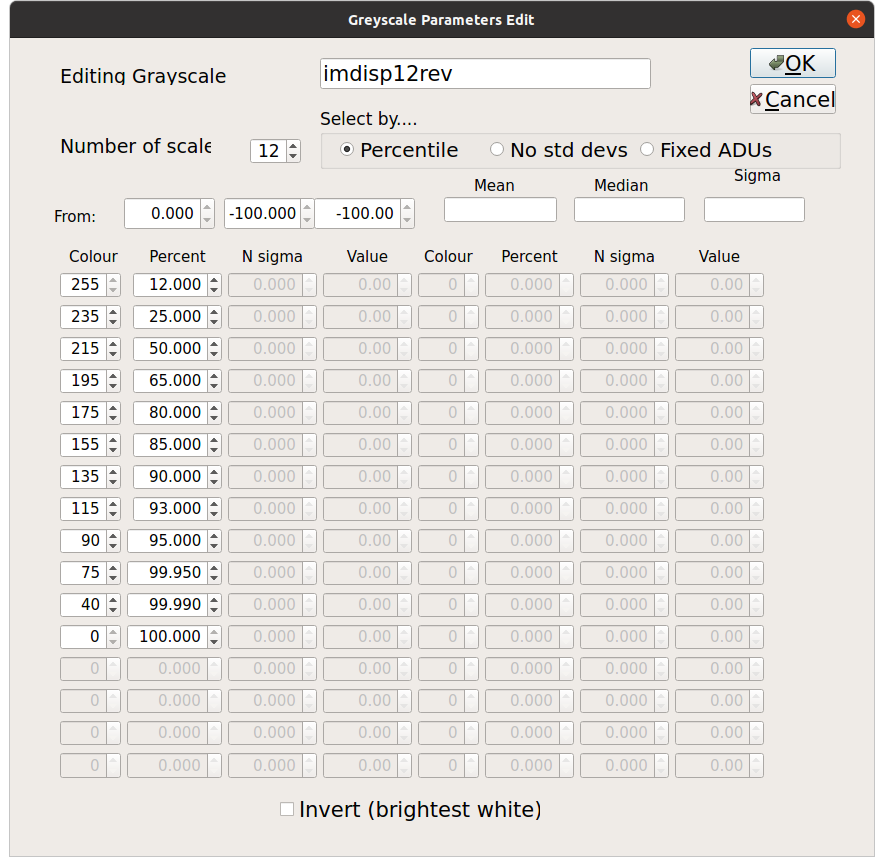
\includegraphics[scale=0.4]{images/geditorshot.png}
\end{center}   
\caption{This illustrates one of the dialogs from the graphical display editor
showing how the grey scales are tuned. Grey scales are assigned using
percentiles of the ADU values (default) by number of standard deviations or
absolute value. The values used are as shown in the figures. If an images is
loaded the other boxes are filled in to show the values from the current image
and updated, along with the figure displayed to show the effect on the image.
The results are saved in a configuration file for future use.}
\protect\label{fig:geditorshot}
\end{figure}

\subsection{Analysis of supplied master calibration files}
\protect\label{section:masterbiasflat}

In order to address the matters such as those referred to in Section
\ref{section:mattersaddressed} above, a study was made of the master bias and
flat files supplied.

The following problems were observed with these files.

\begin{enumerate}
  \item The number of daily bias or flat files going to make up the master files
  is not consistent, month by month. Each master file is made up entirely from
  the daily files for the calendar month concerned, which may vary considerably
  in number and criteria for selection. In Fig. \ref{fig:mastmeanbias} is shown
  the mean value and standard deviation of the master bias files up to March
  2020, showing the net effect.
  \item Some of the criteria for selection of the files, particularly the flat
  files, are unusual and unexplained.\footnote{The selection of the daily flat
  files is restricted to those for which the skewness is negative and the
  kurtosis is less than 7.}
  \item Some of the statistics for selection of daily files, notably the flat
  files are incorrectly calculated.\footnote{It did not seem a productive use of
  time to reproduce the programming error and work out the actual but incorrect
  set of daily flat files which went to make up the master flat files.}
  \item The master bias files, as constructed, include some extreme values for
  some pixels which cause values for the image files to go negative when the
  bias file is subtracted. No account is taken of noisy or unreliable pixels.
  \item The daily flat files consist of sets of 3 in decreasing light and the
  median value is taken, the result being then normalised. This causes the
  benefit of the brighter flat files, with their better signal to noise ratio to
  be ignored in addition to the other ones.
\end{enumerate}

\begin{figure}[!htbp]
\begin{center}
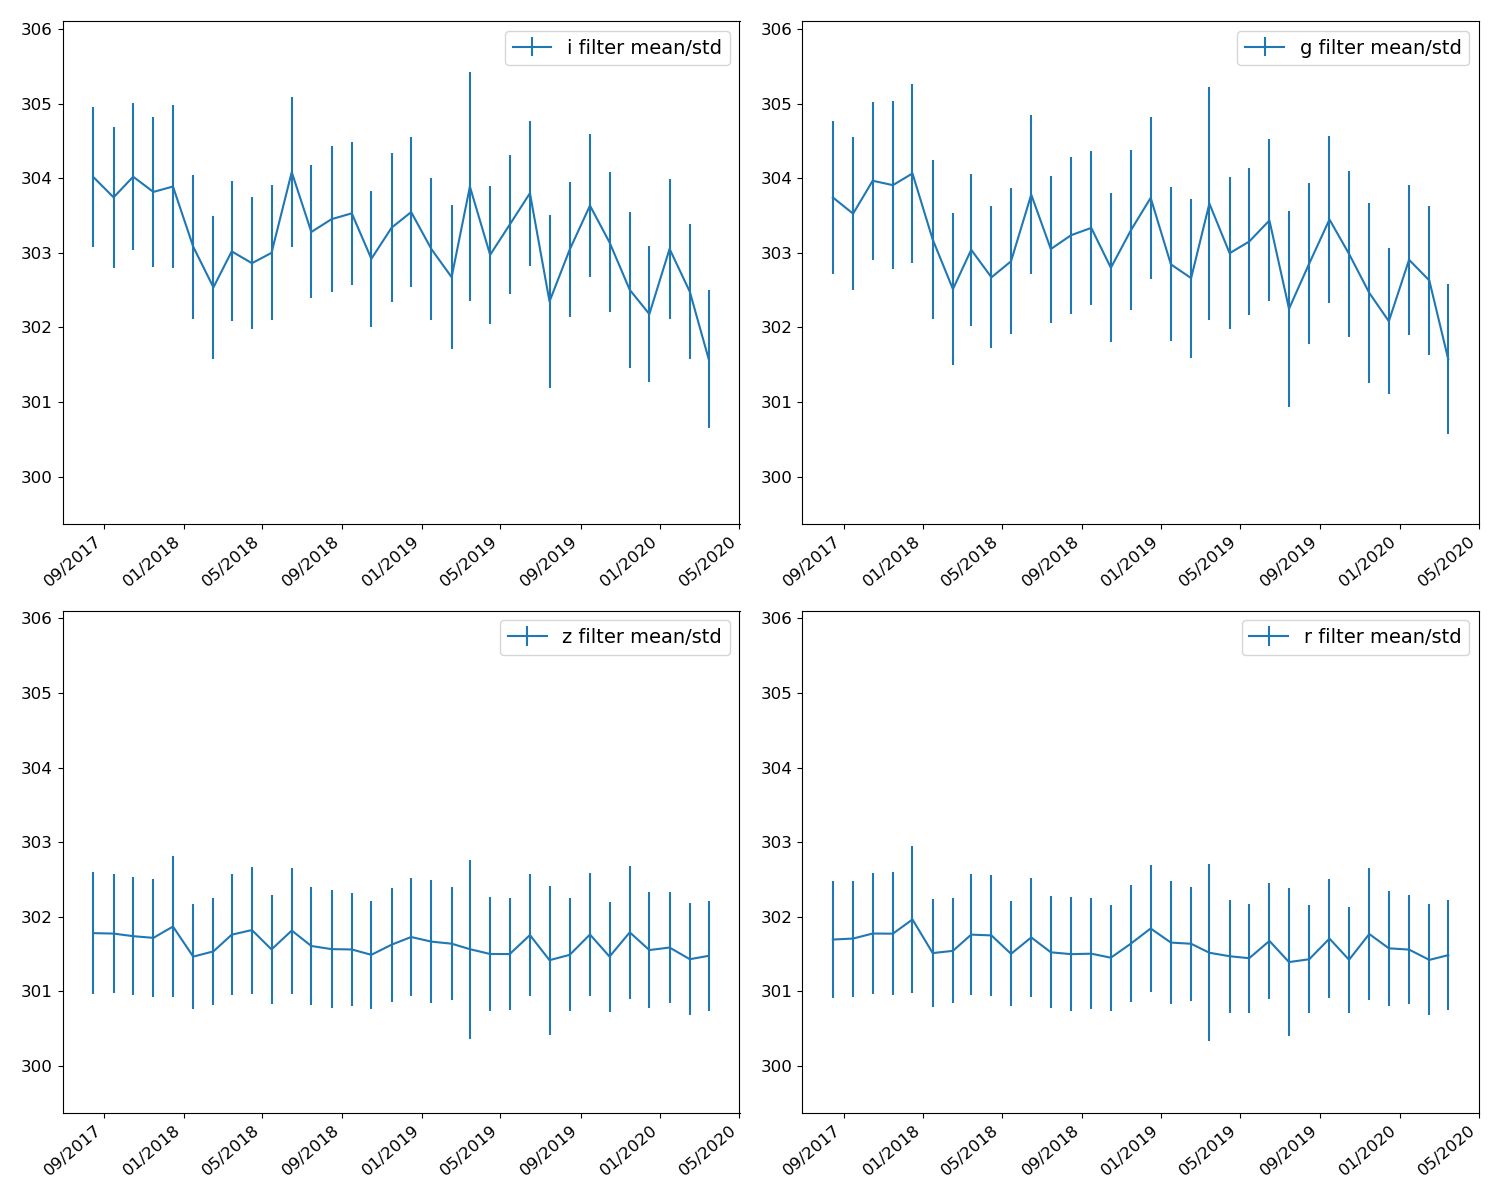
\includegraphics[scale=0.4]{images/mastmeanbias.png}
\end{center}   
\caption{This illustrates the mean and the standard deviation of the values in
the master bias files from July 2017, when {\rdwarf} targets were first
observed, until March 2020.}
\protect\label{fig:mastmeanbias}
\end{figure}
\clearpage

\subsection{Construction of alternative master bias and flat files}
\protect\label{section:altcalib}

Having considered and tried to use the supplied master bias and flat files, I
decided to construct alternative ones from the daily bias and flat files
provided.

A key element in this was to construct the files using a rolling ``window'' of
the same number of daily files centred on the relevant date. This made a
substantial difference to the resulting master files, all of the variations
seen in Fig. \ref{fig:mastmeanbias} from month to month were eliminated and the
resulting files were very similar.

\subsubsection{Defective or unreliable pixels}
\protect\label{section:badpix}

I undertook a study of all the files, flat files, bias files and observation
files to determine whether any pixels in the CCD array could be counted as
``bad'' or unresponsive, had particularly high mean values or large standard
deviation. The literature varies somewhat on how bad pixels are defined or
determined.

\Notnow{Of recent papers, \citet{allers20} define bad pixels as ``dead'' pixels or pixels
with an uncertainty in the flat fields of over 10\%. In \citet{piskunov20} bad
columns in the CCD used are first identified and eliminated and then an
iterative procedure is adopted to effectively assign weights to each pixel. In
\citet{bongiovanni19} a procedure based on constructing two composite flat
fields from low and high counts and regarding as bad the pixels where the ratios
differ by more than 15\%. In \citet{belli18} a bad pixel mask is constructed by
selecting pixels in the flat fields with very low counts and those in the dark
frames with very high counts (but the criteria for ``low'' and ``high'' counts
in those files are not defined). In \citet{briesemeister18} pixels in the
constructed flat fields with values less than 0.5 or greater than 1.5 are
considered to be bad.

A comprehensive study of the quality of pixels is described in the
recently-published \citet{maslennikova20}. Pixels are described as
\textbf{Normal}, \textbf{Cold}. \textbf{Warm}. \textbf{Dead}, \textbf{Hot} and
\textbf{Inverse} according to the responses. The pixels on the ROSS2 telescope
CCD do not fit neatly into these brackets, apart from the \textbf{Normal} ones.}

For the purposes of this study, it was clear that the pixels could be described
as:
\begin{description}
\item[Normal] pixels are those which are clearly well-behaved with a linear
response within 10\% of saturation.
\item[Consistently high] pixels are those which whose count never falls below a
value significantly higher than bulk of the pixels. These are often found in
whole sections of a column on an array.
\item[Noisy] pixels are closest to \textbf{Dead} pixels as defined in 
\citet{maslennikova20}. Included are those with consistent high levels of noise,
with the standard deviation on the bias level over 5 times the standard
deviation.
\item[Bad] pixels are ones which give random readings, usually very low ones.
\end{description}

In addition, all of the pixels, to a greater or lesser extent, can give random
very high readings which stand out from the neighbouring pixels. These might
perhaps be due to cosmics in some cases, or because on resetting the CCD those
pixels are not reset. Some are random much more often than others and these
correspond to the \textbf{noisy} pixels.

There are very few examples, in the order of 25 pixels spread over the used area
of the array, which qualify as \textbf{bad}.

It is straightforward to interpolate over the relevant pixels. There are a few places where there are strings of
adjacent noisy or consistently high pixels, but these almost entirely affect
columns in the CCD, the worst example can be found in the area used for the \gfilter, seemingly as
the CCD is read out by columns, so adjacent pixels on the same row have to be
used for interpolation.

\subsubsection{New master flat and bias files}
\protect\label{section:newmastfb}

With appropriate adjustments for the defective pixels as described above, it
proved straightforward to construct new master bias files using a  ``rolling
window'' centred on the date required. I constructed standard deviations for each individual pixel.

I made an extensive study of the linearity using the daily flat
files; it would  appear than the performance is linear up to 62,000 counts per
pixel out of a possible 65,536. I constructed the master
flat files using daily files with pixels between a range of 5,000 and 61,000 to be clear of this linearity cut-off.
None of the image files, other than ones contaminated by cosmics and similar,
had pixel values close to 60,000. I did not use the skewness or kurtosis
measurements used in the construction of the original master flat files as this
did not seem to have any benefit\footnote{Even if they were correctly
calculated.}. I then subtracted from the selected daily flat files
the newly-constructed master bias file centred on the relevant date and normalised the result.
I then combined the results into a master flat file for the relevant date using a weighted geometric mean,
the weights being inversely proportional to the standard deviations.

This resulted in a much more satisfactory set of master bias and flat files and
it was possible to much more confident of the uncertainty of values on a
per-pixel basis. The combination of the flat files using a weighted
geometric mean, included many more of the brighter files, with their higher
SNR, giving them priority over the darkest files, whilst still obtaining some
benefit from the latter.

When the object ADU counts from {\rem} images are computed from the images, the
standard deviations for each individual pixel in the image are combined into an
overall standard deviation for the ADU count for the relevant object.

\subsection{Finding and identifying objects}
\protect\label{section:findingidentify}

Most of the objects in the neighbourhood of the target {\rdwarf} objects were
identified using GAIA DR3. Where alternative shorter names than GAIA DR3 nnnnnnn
were found, this was used in preference. Bearing in mind the resolution of the
{\rem} telescope of around 0.6 arcsecond, objects closer together than this
distance were eliminated, as were objects with irregular profiles and one marked
as variable.

The magnitudes in various bands are all noted in the database records, but these
were mainly used as a guideline where there was ambiguity in distinguishing
close but not overlapping objects. It proved better to explicitly count the ADUs
after adjusting the aperture sizes.

There remains considerable work in finalising the optimal aperture sizes for
each objects, particularly with {\prox} and {\bstar}.

The best frames contain up to 200 possible reference stars for the best
examples, more for {\prox} and less for {\bstar}. Average frames contain up to
30 or so. Any less than 10 are rejected as too poor in contrast, but the total of rejected frames is less than
10\%.\footnote{This figure is subject to amendment, currently the rejection is
binary, but there is provision for a ``quality'' marker enabling frames to be
partially used where appropriate.}

\subsection{Calibration of reference stars and ADU counts}
\protect\label{section:calibrationrefstars}

Not all the frames contain the same reference stars, or have the same
orientation, some are rotated by 90\degree or 180\degree relative to others. The
target object may be off-centre by varying amounts and in varying directions and
different reference objects appear in different frames, or are too close to the
edge in some cases, where vignetting or similar reduces the accuracy, to be
usable. Only quite a small handful of objects appear in all the frames.

After some experimentation with strategies for computing and calibration of the
objects, the most promising strategy emerged as being for each filter
(initially this was only done with the {\rfilter} images, being the least
problematic).

\begin{enumerate}
  \item Compute the ADU count and standard deviation for each object in each
  frame.
  \item Compute the mean ADU count and corresponding standard
  deviation for each object. Clearly strongly variable objects previously missed can be weeded out
  at this stage.
  \item For each observation, perform a linear regression fit of the calculated
  ADUs for each object other than the target in the frame to the mean ADUs.
  \item Apply the fit backwards, propagating the standard deviation, to the
  calculated ADUs for the target on the frame and compare with the mean ADUs for
  the target to give the variation from the mean of the target for that frame.
\end{enumerate}

This technique proved very successful, in most cases the correlation of the
linear regression was better than 95\%, and proved insensitive to what set of
reference stars were available on a particular frame.

\subsection{Results for \ross}
\protect\label{section:resultsross}

The results for {\ross} are set out in the draft paper attached to this report.
but in summary the data sources referred to in papers which mentioned
measurements for {\ross} were studied and a rotation period of $2.87 \pm 0.01$
days was confirmed consistently.

After processing the data using the modified bias and flat files and processing
the counts relative to the reference stars as described above in Section
\ref{section:calibrationrefstars}, the period of 2.87 days was clearly extracted
from the data.

This confirms that there is viability in the methods used in terms of recovering
the rotation period for \ross. More challenging may be that for \bstar, where
the number of observations is less and also the number of reference objects.

\subsection{Set up of pipeline}
\protect\label{section:pipeline}

A daily routine was set up to interrogate the {\rem} results and load new data
into the database. The steps were:

\begin{enumerate}
  \item Load information about new observations into the database. This is just
  a simple record of information.
  \item Load FITS files corresponding to the ROSS2 observations of the target
  objects into the database cache.
  \item For loaded FITS files, add data about statistics such as maximum and
  minimum pixel values, mean and standard deviations into the database.
  \item For database rows corresponding to the targets, compute the barycentric
  dates and add to the database.
  \item Identify the target and other objects in the frames and add locations to
  the database. Mark frame as too poor to use if the target is not found, and
  less than a given number of reference objects, currently 10, are not found.
  \item Load FITS files corresponding to daily flat and bias files into the
  database.
  \item Load any new master bias and flat files (although these are no longer
  used).
\end{enumerate}

The calculation of ADUs for objects is currently done manually when ready, but
ultimately this will be added to the pipeline. Currently the daily job takes
about 40 minutes to run.
